%&latex
\documentclass{article}

 
\usepackage{amsthm}
\newtheorem{definition}{Definition}

\usepackage{outlines}
\usepackage{enumitem}
\setenumerate[1]{label=\arabic*.}
\setenumerate[2]{label=\alph*.}
\setenumerate[3]{label=\roman*.}
\setenumerate[4]{label=\alph*.}

\usepackage{graphicx}
\DeclareGraphicsRule{.tif}{png}{.png}{`convert #1 `dirname #1`/`basename #1 .tif`.png}


\begin{document}

%+Title
\title{Introduction to Databases and DBMS}
\author{DSC 301}
\date{\today}
\maketitle
%-Title

 

% ---------------- %
% \begin{outline}[enumerate]
% 	outline (enumeration) template
% \end{outline}
% ---------------- %
% \begin{outline}
% 	itemize template       
% \end{outline}
% ---------------- %
%\begin{definition}
% 	defintion template
%\end{definition}













% --------- Lecture Objectives ------- %
\section*{Objectives}
\begin{outline}
     \1 Why databases are important?
     \1 What is a database?
     \1 What are the common Databases
     \1 What role associated with database environments
     \1 Types of databases  
     \1 Features of databases
     \1 Database Architecture  
\end{outline}

% Database Architecture













% -------- Why are databases important? -------- %
 \section{Why are databases important?}
  
Databases have become ubiquitous in society.  Annual sales from the database market is approximately \$50 billion (and growing).  

% ---------------- %
\begin{outline}
   \1 Most important development in software engineering
   \1 Underlying framework of information systems
   \1 Fundamentally changed the way organizations operate
   \1 Backbone of the web
        \2 Nearly all website have backend databases driving content
                \3 WordPress (CMS), Joomla, Blackboard
                \3 Amazon (online store), Facebook, IRS, 
                \3 Online banking, travel (airline reservations)       
   \1 Every business leverages databases (employees, tax records, etc.)
\end{outline}








\newpage


 
 % -------- Data is important -------- %
 \subsection*{Data is important}
\begin{outline}
    \1 Data is new oil.
        \2 Oil and energy companies dominated the top of the valuable firms in the world until around 2016.  
        \3 Alphabet, Apple, Facebook, Amazon, and Microsoft
        
    \2 If the product is free, then YOU are the product.  
    
    
\end{outline}

\subsection*{The 5V's of data}



% ---------------- %
\begin{outline}[enumerate]
        \1 \textbf{Volume} - In the digital universe there is $\approx 45$ zettabytes ($10^{21}$)

        \1 \textbf{Velocity} - high rate of data collection.
                \2 95 million photos and videos shared daily on Instagram
                \2 305 billion emails per day
                \2 5 million Tweets per day
                \2 3.5 billion Google searches per day
                
                
        \1 \textbf{Variety} - data can be structured data, semi-structured, unstructured.  Also data comes from a variety of sources and can be highly heterogeneous.  


        \1 \textbf{Veracity} - data is inaccurate, inconsistent, and difficult to maintain.  High dimensionality with data.  Missing data????


        \1 \textbf{Value} - data is meaningless.  Only if information can be extracted makes it valuable.  For example, clickstream are sequences of user interactions with a website.  A data scientist wants to convert these clickstreams into actionable information.  
\end{outline}






% ----- What is a database ----- %
\section{What is a database?}
\begin{definition}
        A \textbf{database} is any collection of related data organized for systematic management.
\end{definition}

\subsection*{Examples of database}

 \begin{outline}
        \1 Notebook containing a list of friends and family.
        \1 Box of recipes
        \1 Filing cabinet
        \1 Spreadsheet
        \1 Expense ledger
\end{outline}
However, we think of databases as ``electronic database"



\newpage

\begin{definition}
        A \textbf{database} refers to an electronic database managed by software.  \textbf{Database Management System} (DBMS) is software used to create, store, retrieve, modify, and delete data in conjunction with various data-processing operations such as generating reports, printing invoices, etc.  
\end{definition}


There are many DBMS.  Here are a few:
% ---------------- %
\begin{outline}
        \1 Microsoft SQL Server (MS SQL Server)
                \2 American Airlines
        \1 PostgreSQL
        \1 Amazon RDS
        \1 Oracle RDBMS
        \1 IBM Db2 (and Informix)
        \1 SAP Sybase
        \1 Apache (open-source foundation) Cassandra (Big Data)
                \2 Apple, Constant Contact, Comcast, eBay, Hulu, Macy's Microsoft, McDonalds, Netflix, New York Times, Uber, Walmart

        \1 Google Cloud BigTable (NoSQL)
        
        \1 MongaDB
        
        \1 \textbf{MySQL} 
                \2 LinkedIn, Etsy, Twitter, Uber, Tesla, Toyota, Netflix, Verizon, Bank of America, PayPal, Pinterest, Yahoo, YouTube, Google, Facebook, Yelp, Dropbox, Github, Airbnb, ...
        \2 LAMP  - Linux (OS), Apache - Webserver, M-MySQL, P=php or perl or Python.  

        \2 WordPress, Online Shopping, etc.  
                
\end{outline}




\section*{Key Features of a DBMS}
 \begin{outline}[enumerate]
  \1 Allows users to create new and multiple databases
  \1 Provide ability to access, retrieve, and update data
  \1 Supports storage of large amounts of data
  \1 Control who access and different levels of access
  \1 ACID Transaction management
        \2 A = Atomicity - transaction is ``all or nothing"
        \2 C  = Consistency - only valid data will be written to the database.  Sum of balances must be equal (Credit = Debit)
 
        \2 I = Isolation - multiple transactions cannot interfere
        \2 D = Durability - a transaction will endure (will not be lost).  Also provides a mechanism for back-up and recovery.

  \end{outline}
Google to get additional perspectives on these concepts.  




\subsection*{Database Architecture}
Components of the DBMS:

\begin{outline}
        \1 Storage Manager
        \1 Concurrency controller (manager)
        \1 Query language compilers
                \2 DDL = Data definition language (create databases, etc.)
                \2 DQL = Data query language (retrieve data)
                \2 DML  = Data Manipulation language (update/modify the data)
        \1 Recovery engine
        \1 Buffer manager
        \1 Authorization manager
        \1 Transaction manager
        
\end{outline}





\section*{Client-server Model}
\begin{outline}
        \1 Two-tier
                \2 Client $\to$ Database (Server)
         \1 Three-tier 
                \2 Client $\to$ Application Server $\to$ Database server
                \2 Client $\to$ Web Server $\to$ Database server
\end{outline}


\newpage

 

\begin{figure}[h!]
 \centering
     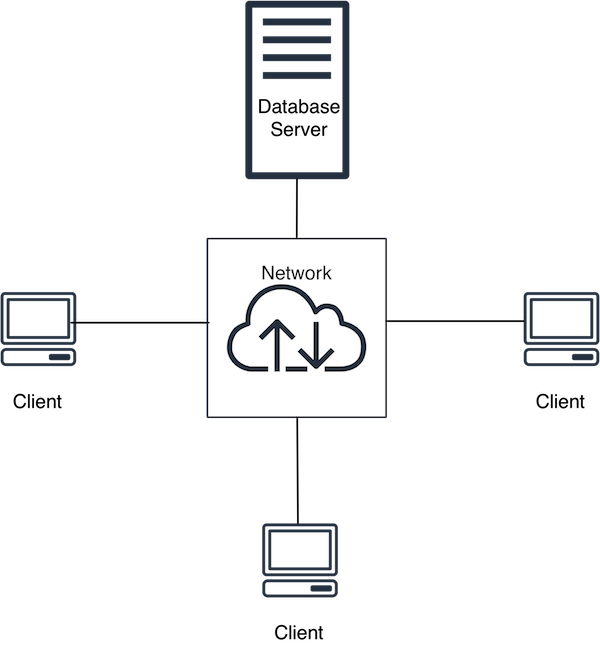
\includegraphics[width=0.6\textwidth]{figs/Client_Server.png}
    \caption{Two-tier client-server model.}
    \label{fig:dbarc2}
\end{figure}

 







  
%+Bibliography
%\begin{thebibliography}{99}
%\bibitem{Label1} ...
%\bibitem{Label2} ...
%\end{thebibliography}
%-Bibliography



 

\end{document}
